\documentclass{pbpreprint}
\usepackage{listings}

\newsubfloat{table}

\begin{document}

\pretitle{\begin{center}
\includegraphics[width=8em]{figures/UU_logo.pdf}\todo{Consider how much space we want above}\\\Huge\bfseries}
\title{The pharm\textcolor{uured}{b.io} preprint class}
\posttitle{\par\vskip1em{\normalfont\LARGE\scshape QSAR\par}\end{center}}
\maketitle
\section*{About the class}
This is the pharm\textcolor{uured}{b.io} preprint class. It is meant to be used
for setting articles in a consistent way for preprint purposes but could also
be used for teaching materials an similar things. It uses the EB Garamond
font\footnote{See: \url{http://www.georgduffner.at/ebgaramond/}}. In the
projects own words: ``EB Garamond is an open source project to create a revival
of Claude Garamont’s famous humanist typeface from the mid-16th century.''

The class has a macro for making margin notes\note{This is a margin note //jonalv} and
another for making todos\todo{write what to do here}. 

It also uses EB Garamond for math type setting as can be seen here:
\begin{equation}
    \int_{a}^{b} x^2 dx
\end{equation}

\section*{Some tips on the way}
The EBGaramond font contains both old style (\oldstylenums{0, 1, 2, 3, 4, 5, 6,
7, 8, 9}) numbers and lining numbers (\liningnums{0, 1, 2, 3, 4, 5, 6, 7, 8,
9}) default is old style. There is also tabular and propotional numbers where
tabular numbers are good for aligning numbers in tabels (see
Table~\ref{tabular}). 


\begin{table}[h]
    \caption{Comparison of tabular nums and proportional numbers}
    \hfill
    \subtop[Tabular\label{tabular}]{\tabularnums{
        \begin{tabular}{lrr}
            \toprule
            Letter & Number & Number \\
            \midrule
            a &    123 &       45 \\
            b &     12 &        6 \\
            c & 1\,000 & 100\,000 \\
            d & 5\,000 & 123\,000 \\
            \bottomrule
        \end{tabular}
    }}
    \hfill
    \subtop[Proportional]{
        \begin{tabular}{lrr}
            \toprule
            Letter & Number & Number \\
            \midrule
            a &    123 &       45 \\
            b &     12 &        6 \\
            c & 1\,000 & 100\,000 \\
            d & 5\,000 & 123\,000 \\
            \bottomrule
        \end{tabular}
    }
    \hfill
\end{table}

\lstset{language=Tex, basicstyle=\ttfamily\scriptsize}
\begin{figure}
\begin{minipage}{0.49\textwidth}
\begin{lstlisting}
\begin{figure}
    \begin{center}
    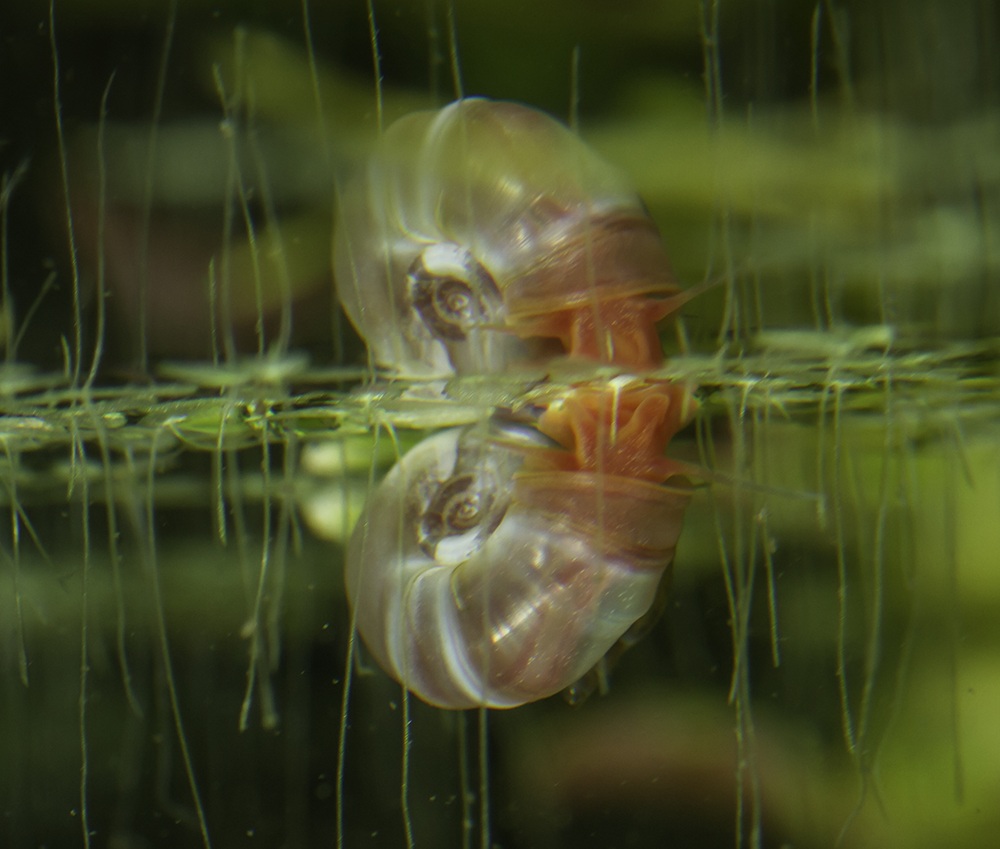
\includegraphics
      [width=0.7\textwidth]
      {figures/snail.png}
    \end{center}
    \caption{Snail on water surface}
\end{figure}
\end{lstlisting}
\end{minipage}
\hfill
\begin{minipage}{0.49\textwidth}
\begin{lstlisting}
    \begin{figure}
        \centering
        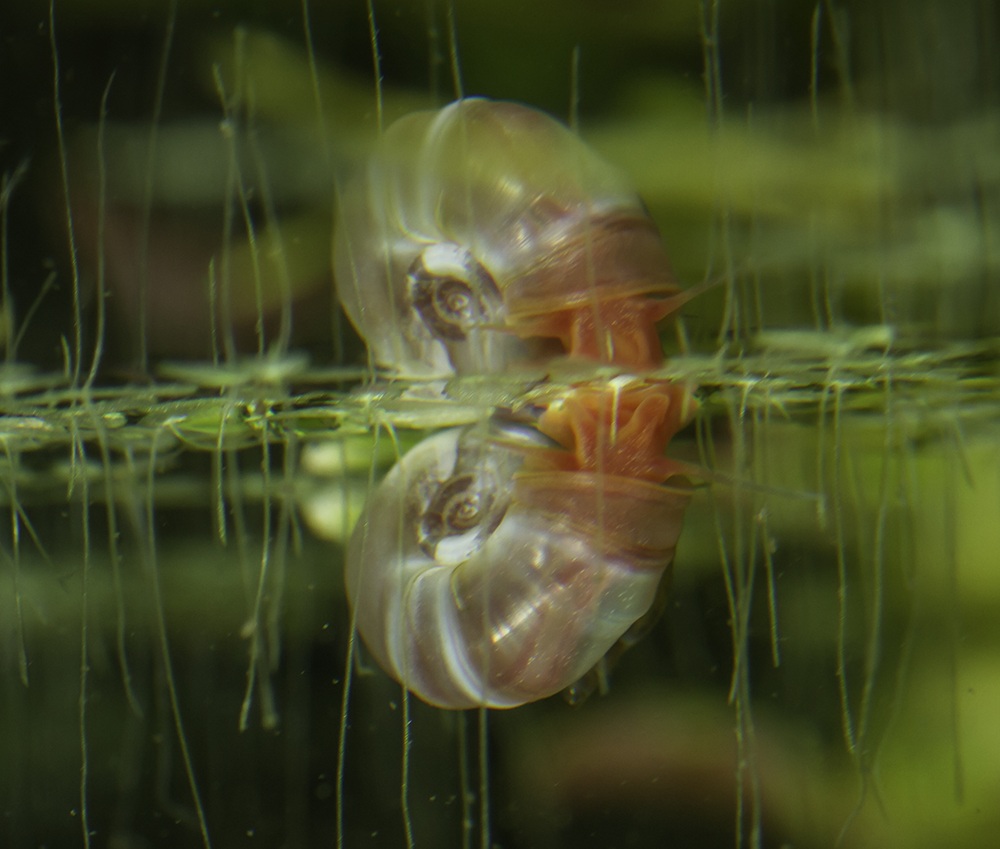
\includegraphics
          [width=0.7\textwidth]
          {figures/snail.png}
        \caption{Snail on water surface}
    \end{figure}
\end{lstlisting}
\end{minipage}

\fbox{\begin{minipage}[t]{0.44\textwidth}
    \begin{figure}[H]
        \begin{center}
        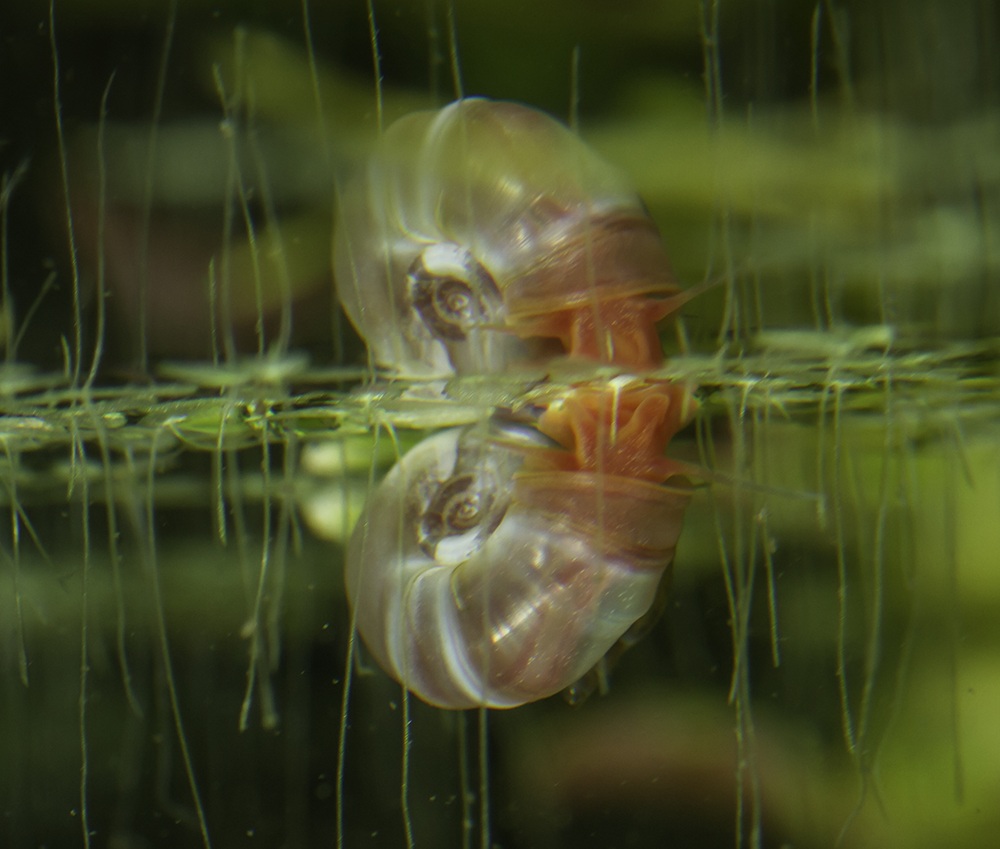
\includegraphics
          [width=0.7\textwidth]
          {figures/snail.png}
        \end{center}
        \caption{Snail on water surface}
    \end{figure}
\end{minipage}}
\hfill
\fbox{\begin{minipage}[t]{0.44\textwidth}
    \begin{figure}[H]
        \centering
        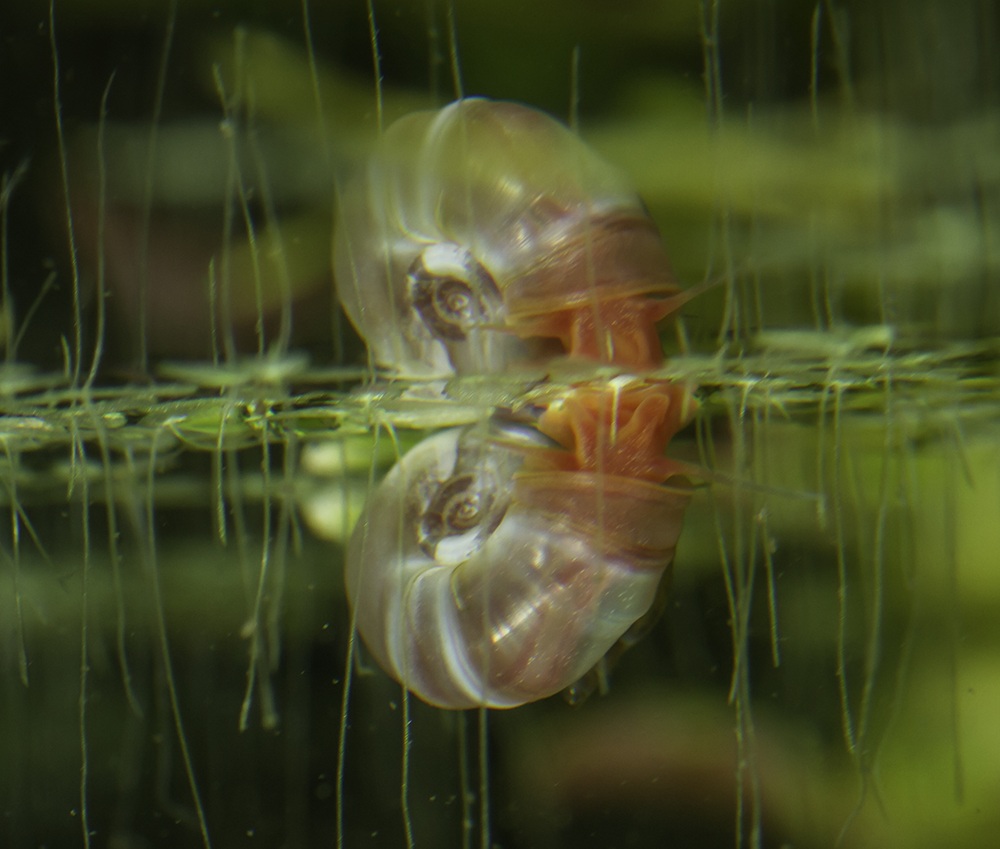
\includegraphics
          [width=0.7\textwidth]
          {figures/snail.png}
        \caption{Snail on water surface}
    \end{figure}
\end{minipage}}
\caption{In \texttt{\textbackslash figure} and \texttt{\textbackslash table} use \texttt{\textbackslash centering} instead of \texttt{\textbackslash begin\{center\}} because othewise you are adding extra space that shouldn't be there. Also, figure numbering is strange here because in order to show the extra space I wanted to use real figures which end up with their own numbers.}
\end{figure}

\end{document}
